% Generated by pysimcount.pfboundchilds -- do not edit; regenerate instead.
% figure: bound-min-t-all-formulas -- Every formula, X-Y-Z grouping, T gates vs n, r from the minimised norm bound (every step synthesised)
% r from minimised norm bound (Childs et al. 2018, Def. 2; extended to every formula); bound settings {"kind": "min", "budget": "count", "constant": "childs"}
% NumPy seeds [1, 2, 3, 4, 5, 6, 7, 8, 9, 10]; t = n; sizes [4, 5, 6, 7, 8, 9, 10, 11, 13, 20, 30, 50, 70, 100, 200, 300, 500]; ct: eps_trotter = 0.0005, eps_synth = 0.0005, merged, simcount template, pygridsynth
% one step built and synthesised per formula, seed and n, eps_rot = eps_synth / (rotations x r)
% formulas as in bound-min-cnot-all-formulas.json (pruning not re-run)
% shown: suzuki2, suzuki4, mo-q6, mo-q14, bm-q10, mo-o8-q21, morales-y8m10, morales-m8
% removed: lie-trotter, suzuki6, suzuki8
% figure made at git_commit=eed0c490bd2a7ed3c821acf76ae930c79d2195f6 git_dirty=True
% WARNING: made from uncommitted code; the commit above does not reproduce it.
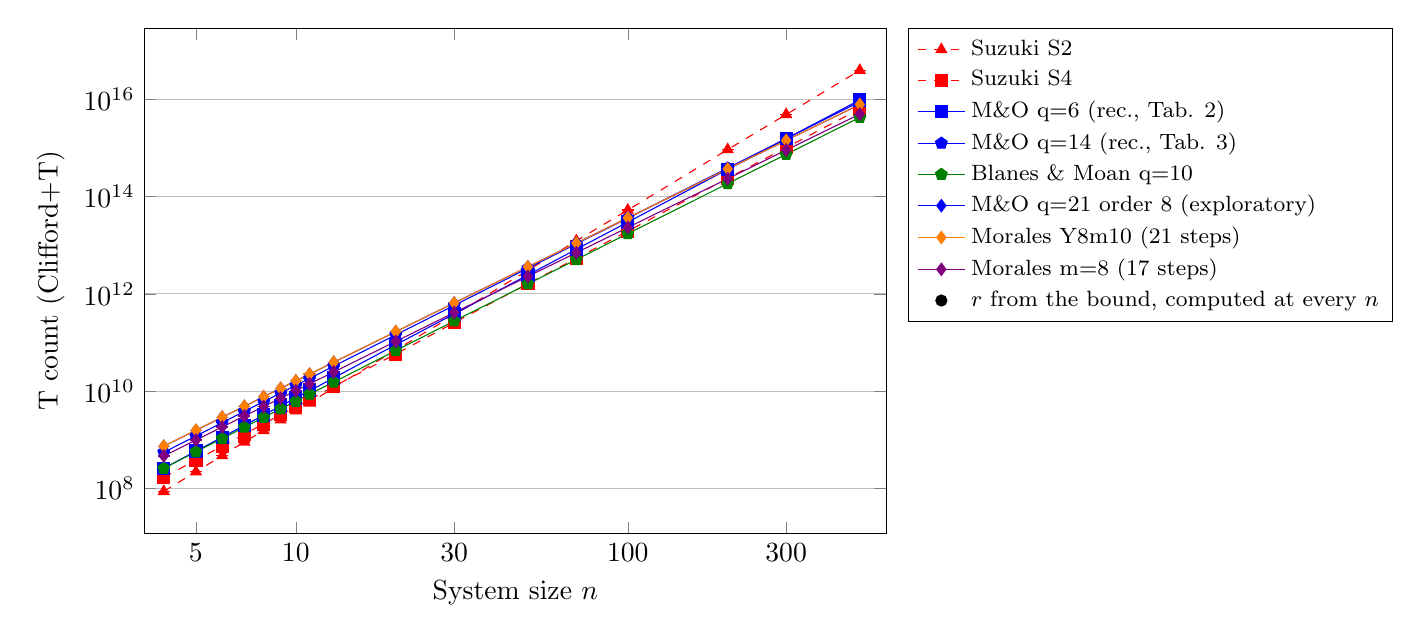
\begin{tikzpicture}
  \begin{loglogaxis}[
    width=11cm, height=8cm,
    xlabel={System size $n$},
    ylabel={T count (Clifford+T)},
    xtick={5,10,30,100,300}, xticklabels={5,10,30,100,300},
    xmin=3.5, xmax=600,
    ymajorgrids=true,
    legend pos=outer north east,
    legend cell align=left,
    legend style={font=\footnotesize},
  ]
    % suzuki2: r from the bound at every n; point = mean over seeds, bars min..max over seeds
    \addplot[red, dashed, mark=triangle*, mark size=2.2pt, mark options={solid, fill=red}, error bars/.cd, y dir=both, y explicit, error bar style={solid}] coordinates {
      (4,8.62687e+07) += (0,254701) -= (0,194771)
      (5,2.19039e+08) += (0,643544) -= (0,819056)
      (6,4.70263e+08) += (0,1.23813e+06) -= (0,530628)
      (7,9.00087e+08) += (0,962832) -= (0,1.44425e+06)
      (8,1.54747e+09) += (0,2.15558e+06) -= (0,3.23337e+06)
      (9,2.55535e+09) += (0,2.89838e+06) -= (0,3.06888e+06)
      (10,3.94935e+09) += (0,5.14481e+06) -= (0,5.37867e+06)
      (11,5.6951e+09) += (0,9.95973e+06) -= (0,8.71476e+06)
      (13,1.17213e+10) += (0,1.66952e+07) -= (0,2.44007e+07)
      (20,6.95434e+10) += (0,6.5457e+07) -= (0,9.351e+07)
      (30,3.68634e+11) += (0,3.18716e+08) -= (0,3.12405e+08)
      (50,3.03699e+12) += (0,1.60687e+09) -= (0,2.19119e+09)
      (70,1.2311e+13) += (0,3.60743e+09) -= (0,6.01239e+09)
      (100,5.28099e+13) += (0,1.22698e+10) -= (0,2.62925e+10)
      (200,9.27206e+14) += (0,1.92571e+11) -= (0,2.84183e+11)
      (300,4.86931e+15) += (0,6.08906e+11) -= (0,5.89976e+11)
      (500,3.9433e+16) += (0,5.33124e+12) -= (0,4.16275e+12)
    };
    \addlegendentry{Suzuki S2}
    % suzuki4: r from the bound at every n; point = mean over seeds, bars min..max over seeds
    \addplot[red, dashed, mark=square*, mark size=2.2pt, mark options={solid, fill=red}, error bars/.cd, y dir=both, y explicit, error bar style={solid}] coordinates {
      (4,1.68074e+08) += (0,498813) -= (0,855581)
      (5,3.82183e+08) += (0,599539) -= (0,1.1299e+06)
      (6,7.34359e+08) += (0,1.0359e+06) -= (0,1.32667e+06)
      (7,1.30059e+09) += (0,3.15088e+06) -= (0,2.32311e+06)
      (8,2.1159e+09) += (0,4.77015e+06) -= (0,3.24221e+06)
      (9,3.26505e+09) += (0,3.92557e+06) -= (0,4.82569e+06)
      (10,4.75134e+09) += (0,9.75834e+06) -= (0,4.55389e+06)
      (11,6.64172e+09) += (0,1.06471e+07) -= (0,9.98681e+06)
      (13,1.23961e+10) += (0,2.66806e+07) -= (0,1.65344e+07)
      (20,5.76672e+10) += (0,5.43677e+07) -= (0,5.03268e+07)
      (30,2.55507e+11) += (0,1.57287e+08) -= (0,2.37194e+08)
      (50,1.6134e+12) += (0,7.97367e+08) -= (0,8.69855e+08)
      (70,5.36739e+12) += (0,1.4241e+09) -= (0,3.95303e+09)
      (100,1.94635e+13) += (0,3.95383e+09) -= (0,6.59654e+09)
      (200,2.37836e+14) += (0,4.63863e+10) -= (0,4.04794e+10)
      (300,1.01276e+15) += (0,2.51119e+11) -= (0,1.74858e+11)
      (500,6.36193e+15) += (0,8.36818e+11) -= (0,7.81907e+11)
    };
    \addlegendentry{Suzuki S4}
    % mo-q6: r from the bound at every n; point = mean over seeds, bars min..max over seeds
    \addplot[blue, solid, mark=square*, mark size=2.2pt, mark options={solid, fill=blue}, error bars/.cd, y dir=both, y explicit, error bar style={solid}] coordinates {
      (4,2.57703e+08) += (0,489346) -= (0,422994)
      (5,5.81845e+08) += (0,1.36067e+06) -= (0,1.24487e+06)
      (6,1.1242e+09) += (0,1.82538e+06) -= (0,2.28172e+06)
      (7,1.97549e+09) += (0,2.54798e+06) -= (0,3.4867e+06)
      (8,3.20668e+09) += (0,4.63237e+06) -= (0,4.25804e+06)
      (9,4.94547e+09) += (0,4.20688e+06) -= (0,3.95572e+06)
      (10,7.24806e+09) += (0,6.37141e+06) -= (0,3.43076e+06)
      (11,1.0121e+10) += (0,2.27997e+07) -= (0,1.86543e+07)
      (13,1.8635e+10) += (0,7.09356e+07) -= (0,2.50083e+07)
      (20,8.96775e+10) += (0,7.05769e+07) -= (0,7.24221e+07)
      (30,3.86026e+11) += (0,2.38796e+08) -= (0,2.81982e+08)
      (50,2.43634e+12) += (0,5.55288e+08) -= (0,6.73629e+08)
      (70,8.23766e+12) += (0,1.66709e+09) -= (0,2.97544e+09)
      (100,2.97927e+13) += (0,8.87602e+09) -= (0,6.56053e+09)
      (200,3.62747e+14) += (0,6.51651e+10) -= (0,3.95645e+10)
      (300,1.55103e+15) += (0,2.717e+11) -= (0,3.17384e+11)
      (500,9.67956e+15) += (0,5.50269e+11) -= (0,6.70955e+11)
    };
    \addlegendentry{M\&O q=6 (rec., Tab. 2)}
    % mo-q14: r from the bound at every n; point = mean over seeds, bars min..max over seeds
    \addplot[blue, solid, mark=pentagon*, mark size=2.2pt, mark options={solid, fill=blue}, error bars/.cd, y dir=both, y explicit, error bar style={solid}] coordinates {
      (4,5.50279e+08) += (0,622699) -= (0,1.02783e+06)
      (5,1.18765e+09) += (0,1.337e+06) -= (0,1.94243e+06)
      (6,2.24106e+09) += (0,1.71631e+06) -= (0,1.94772e+06)
      (7,3.83354e+09) += (0,4.14198e+06) -= (0,4.41811e+06)
      (8,6.07395e+09) += (0,4.86155e+06) -= (0,3.0526e+06)
      (9,9.12076e+09) += (0,5.94994e+06) -= (0,5.94994e+06)
      (10,1.30737e+10) += (0,1.51466e+07) -= (0,9.56959e+06)
      (11,1.81679e+10) += (0,2.40555e+07) -= (0,1.55095e+07)
      (13,3.24672e+10) += (0,6.13084e+07) -= (0,2.86106e+07)
      (20,1.42981e+11) += (0,1.20757e+08) -= (0,6.72289e+07)
      (30,5.77661e+11) += (0,1.54099e+08) -= (0,2.06559e+08)
      (50,3.35535e+12) += (0,8.38487e+08) -= (0,6.17407e+08)
      (70,1.06752e+13) += (0,2.26838e+09) -= (0,1.6304e+09)
      (100,3.5985e+13) += (0,5.10165e+09) -= (0,6.83838e+09)
      (200,3.86224e+14) += (0,3.68149e+10) -= (0,6.29063e+10)
      (300,1.55395e+15) += (0,1.27823e+11) -= (0,1.41186e+11)
      (500,8.87764e+15) += (0,5.80449e+11) -= (0,8.95269e+11)
    };
    \addlegendentry{M\&O q=14 (rec., Tab. 3)}
    % bm-q10: r from the bound at every n; point = mean over seeds, bars min..max over seeds
    \addplot[green!50!black, solid, mark=pentagon*, mark size=2.2pt, mark options={solid, fill=green!50!black}, error bars/.cd, y dir=both, y explicit, error bar style={solid}] coordinates {
      (4,2.57673e+08) += (0,248489) -= (0,309343)
      (5,5.6315e+08) += (0,775830) -= (0,1.01455e+06)
      (6,1.05686e+09) += (0,1.10789e+06) -= (0,977550)
      (7,1.80445e+09) += (0,1.69828e+06) -= (0,2.0342e+06)
      (8,2.87407e+09) += (0,2.41957e+06) -= (0,2.67427e+06)
      (9,4.3031e+09) += (0,3.01572e+06) -= (0,4.69112e+06)
      (10,6.1567e+09) += (0,3.25493e+06) -= (0,5.31067e+06)
      (11,8.65086e+09) += (0,1.35289e+07) -= (0,6.7912e+06)
      (13,1.52563e+10) += (0,3.49582e+07) -= (0,1.55457e+07)
      (20,6.80439e+10) += (0,3.72452e+07) -= (0,3.16476e+07)
      (30,2.75827e+11) += (0,7.1442e+07) -= (0,7.25496e+07)
      (50,1.59131e+12) += (0,5.35517e+08) -= (0,2.84152e+08)
      (70,5.06469e+12) += (0,9.45811e+08) -= (0,1.84772e+09)
      (100,1.72869e+13) += (0,1.78736e+09) -= (0,2.06234e+09)
      (200,1.8438e+14) += (0,1.4026e+10) -= (0,2.7037e+10)
      (300,7.38404e+14) += (0,1.15202e+11) -= (0,1.05701e+11)
      (500,4.24434e+15) += (0,3.04117e+11) -= (0,4.77675e+11)
    };
    \addlegendentry{Blanes \& Moan q=10}
    % mo-o8-q21: r from the bound at every n; point = mean over seeds, bars min..max over seeds
    \addplot[blue, solid, mark=diamond*, mark size=2.2pt, mark options={solid, fill=blue}, error bars/.cd, y dir=both, y explicit, error bar style={solid}] coordinates {
      (4,7.34481e+08) += (0,511034) -= (0,749958)
      (5,1.55769e+09) += (0,1.38558e+06) -= (0,1.07889e+06)
      (6,2.90479e+09) += (0,1.69888e+06) -= (0,1.51745e+06)
      (7,4.86765e+09) += (0,2.44822e+06) -= (0,1.86531e+06)
      (8,7.64197e+09) += (0,3.8236e+06) -= (0,6.5615e+06)
      (9,1.13807e+10) += (0,4.14092e+06) -= (0,3.03394e+06)
      (10,1.61814e+10) += (0,6.51912e+06) -= (0,6.20745e+06)
      (11,2.22474e+10) += (0,1.95609e+07) -= (0,1.48637e+07)
      (13,3.90543e+10) += (0,8.49347e+07) -= (0,1.90097e+07)
      (20,1.66264e+11) += (0,6.59301e+07) -= (0,5.36067e+07)
      (30,6.50208e+11) += (0,2.73974e+08) -= (0,2.71522e+08)
      (50,3.58857e+12) += (0,6.75107e+08) -= (0,3.87293e+08)
      (70,1.10564e+13) += (0,1.05747e+09) -= (0,1.86395e+09)
      (100,3.6558e+13) += (0,1.02735e+10) -= (0,6.09987e+09)
      (200,3.69357e+14) += (0,3.10001e+10) -= (0,4.56832e+10)
      (300,1.42755e+15) += (0,8.49399e+10) -= (0,1.02611e+11)
      (500,7.82549e+15) += (0,7.44269e+11) -= (0,6.18116e+11)
    };
    \addlegendentry{M\&O q=21 order 8 (exploratory)}
    % morales-y8m10: r from the bound at every n; point = mean over seeds, bars min..max over seeds
    \addplot[orange, solid, mark=diamond*, mark size=2.2pt, mark options={solid, fill=orange}, error bars/.cd, y dir=both, y explicit, error bar style={solid}] coordinates {
      (4,7.38042e+08) += (0,633814) -= (0,793098)
      (5,1.56206e+09) += (0,958405) -= (0,1.4513e+06)
      (6,2.90695e+09) += (0,1.1051e+06) -= (0,1.78135e+06)
      (7,4.87222e+09) += (0,3.59073e+06) -= (0,5.73583e+06)
      (8,7.64216e+09) += (0,5.20828e+06) -= (0,5.01946e+06)
      (9,1.13482e+10) += (0,7.37986e+06) -= (0,2.66495e+06)
      (10,1.62306e+10) += (0,8.25929e+06) -= (0,8.36318e+06)
      (11,2.23956e+10) += (0,2.09765e+07) -= (0,1.44133e+07)
      (13,3.91753e+10) += (0,3.14174e+07) -= (0,2.05548e+07)
      (20,1.67039e+11) += (0,1.55028e+08) -= (0,8.40455e+07)
      (30,6.45747e+11) += (0,2.61102e+08) -= (0,1.9552e+08)
      (50,3.60051e+12) += (0,5.63072e+08) -= (0,8.56681e+08)
      (70,1.10209e+13) += (0,1.96888e+09) -= (0,8.29109e+08)
      (100,3.64014e+13) += (0,5.22387e+09) -= (0,3.99472e+09)
      (200,3.70358e+14) += (0,2.28961e+10) -= (0,2.80809e+10)
      (300,1.42803e+15) += (0,6.87325e+10) -= (0,1.23155e+11)
      (500,7.83221e+15) += (0,4.54015e+11) -= (0,4.74185e+11)
    };
    \addlegendentry{Morales Y8m10 (21 steps)}
    % morales-m8: r from the bound at every n; point = mean over seeds, bars min..max over seeds
    \addplot[violet, solid, mark=diamond*, mark size=2.2pt, mark options={solid, fill=violet}, error bars/.cd, y dir=both, y explicit, error bar style={solid}] coordinates {
      (4,4.62885e+08) += (0,780104) -= (0,528796)
      (5,9.82312e+08) += (0,1.48176e+06) -= (0,937440)
      (6,1.82446e+09) += (0,1.60683e+06) -= (0,1.64587e+06)
      (7,3.07124e+09) += (0,2.36332e+06) -= (0,2.23458e+06)
      (8,4.78934e+09) += (0,2.20923e+06) -= (0,2.63122e+06)
      (9,7.15423e+09) += (0,4.76997e+06) -= (0,4.93167e+06)
      (10,1.01945e+10) += (0,4.17918e+06) -= (0,1.11855e+07)
      (11,1.40551e+10) += (0,1.44391e+07) -= (0,1.01759e+07)
      (13,2.46574e+10) += (0,4.37623e+07) -= (0,2.12349e+07)
      (20,1.04923e+11) += (0,9.61261e+07) -= (0,5.06387e+07)
      (30,4.10346e+11) += (0,1.86107e+08) -= (0,1.11181e+08)
      (50,2.27443e+12) += (0,3.52663e+08) -= (0,3.25242e+08)
      (70,6.9995e+12) += (0,1.86748e+09) -= (0,1.06922e+09)
      (100,2.31127e+13) += (0,2.07608e+09) -= (0,2.58968e+09)
      (200,2.33015e+14) += (0,2.9222e+10) -= (0,3.29671e+10)
      (300,9.04384e+14) += (0,3.83419e+10) -= (0,7.27941e+10)
      (500,4.9572e+15) += (0,2.92503e+11) -= (0,2.97895e+11)
    };
    \addlegendentry{Morales m=8 (17 steps)}
    \addlegendimage{only marks, black, mark=*, mark options={solid, fill=black}}
    \addlegendentry{$r$ from the bound, computed at every $n$}
  \end{loglogaxis}
\end{tikzpicture}
